\begin{center}
    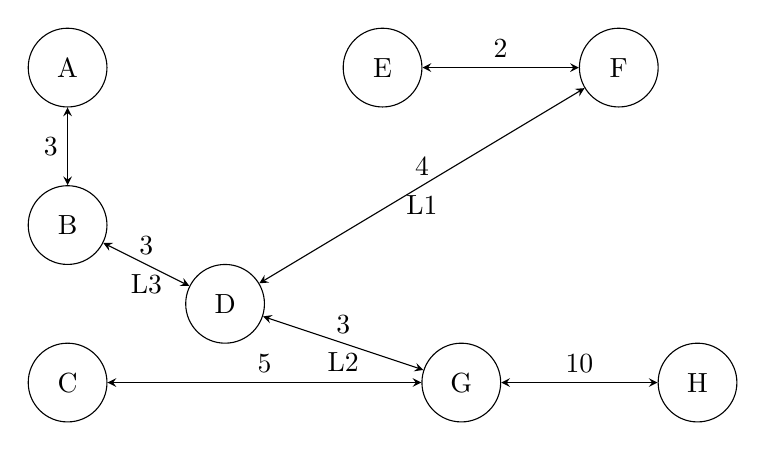
\begin{tikzpicture}
        %%%%%%%%%% Nodi %%%%%%%%%%
        \node[circle, draw, minimum size=1cm] (A) at  (0,4) {A};
        \node[circle, draw, minimum size=1cm] (B) at  (0,2) {B};
        \node[circle, draw, minimum size=1cm] (C) at  (0,0) {C};
        \node[circle, draw, minimum size=1cm] (D) at  (2,1) {D};
        \node[circle, draw, minimum size=1cm] (E) at  (4,4) {E};
        \node[circle, draw, minimum size=1cm] (F) at  (7,4) {F};
        \node[circle, draw, minimum size=1cm] (G) at  (5,0) {G};
        \node[circle, draw, minimum size=1cm] (H) at  (8,0) {H};
        
        %%%%%%%%% Archi %%%%%%%%%%
        \draw[<->,>=stealth] (A) -- node[left] {3} (B);
        \draw[<->,>=stealth] (B) -- node[above] {3} node[below] {L3} (D);
        \draw[<->,>=stealth] (C) -- node[above] {5} (G);
        \draw[<->,>=stealth] (D) -- node[above] {4} node[below] {L1} (F);
        \draw[<->,>=stealth] (D) -- node[above] {3} node[below] {L2} (G);
        \draw[<->,>=stealth] (E) -- node[above] {2} (F);
        \draw[<->,>=stealth] (G) -- node[above] {10} (H);
    \end{tikzpicture}
\end{center}